%-----------------------------------------------------------------------------%
\chapter{\babDua}
%-----------------------------------------------------------------------------%


%-----------------------------------------------------------------------------%
\section{Teori A}
%-----------------------------------------------------------------------------%

\blindtext \cite{Hoffstein1998,Saxena2018,cloud} \\

\begin{figure}
	\centering
	
\includegraphics[width=0.4\textwidth]
	{pics/android-10.jpg}
	\caption{Android 10}
	\label{fig:1}
\end{figure}

%-----------------------------------------------------------------------------%
\section{Teori B}
%-----------------------------------------------------------------------------%

\blindtext \cite{Joshi2015,storage} \\

\begin{figure}
	\centering
	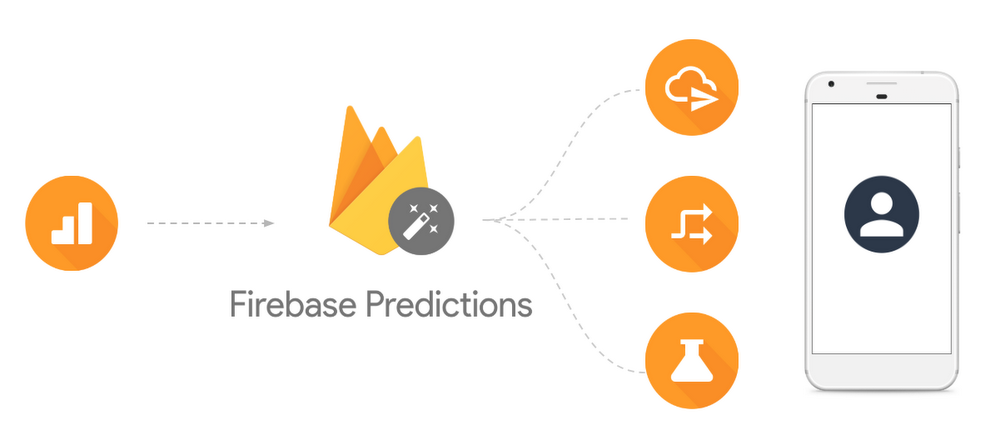
\includegraphics[width=0.8\textwidth]
	{pics/FirebasePre.png}
	\caption{Firebase Prediction}
	\label{fig:2}
\end{figure}

%-----------------------------------------------------------------------------%
\section{Teori C}
%-----------------------------------------------------------------------------%

\blindtext \cite{Mittal2016,uu11} \\

\begin{figure}
	\centering
	
\includegraphics[width=0.6\textwidth]
	{pics/python.png}
	\caption{Python Language}
	\label{fig:3}
\end{figure}

%-----------------------------------------------------------------------------%
\section{Aplikasi Serupa}
%-----------------------------------------------------------------------------%

\blindtext \\

\begin{table}[h]
	\centering
	\caption{Perbandingan Aplikasi Serupa}
	\label{tab:1}
	\begin{tabular}{ c c c }
		\hline
		\textbf{Penulis} 		& \textbf{Aplikasi}  & \textbf{Fitur yang ditawarkan}\\ \hline \hline
		\cite{Narayana2010} 	& Aplikasi-A		& n and p \\ 
		\cite{Patel2016} 		& Aplikasi-B		& p and q \\ 
		\cite{Phadte2017} 		& Aplikasi-C		& q and r \\ 
		\cite{Rachmawanto2017} 	& Aplikasi-D		& r and s \\ 
		\cite{Reddy2016} 		& Aplikasi-E		& s and t \\ \hline
	\end{tabular}
\end{table}